% Do NOT change this "Section" title
% and do NOT add more "Section" level titles.
\section{Method}\label{sec:method}
This section contains the system architecture of the mission control system for Naiad. It also covers the idea behind designing missions for the AUV.

\subsection{System architecture}
The system needed the ability to simultaneously execute missions, receive new missions through the umbilical chord, and communicate with the other systems of the AUV. In order to do this, several tasks were set up.


The new missions needed to be received using Transmission Control Protocol (TCP), so a task was created to handle this. Missions need to communicate with the rest of the AUV through a Controller Area Network (CAN), so two tasks were created to handle the input and output over CAN. Finally, a main task was created to run a virtual machine (VM) which would execute the actual missions. The workflow between these tasks can be seen in \cref{fig:data_flow_figure} along with the resources they use. The TCP resource allows the software to use the Ethernet port on the hardware. The CAN resource allows the software to communicate through the CAN bus on the AUV.

\pageref{fig:data_flow_figure}
\begin{figure}[h]
    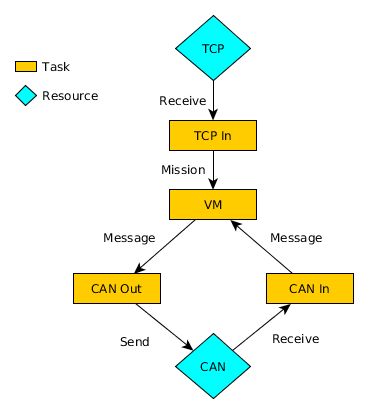
\includegraphics[width=0.5\textwidth]{./figure/figureTasksAndResources.png}
    \caption{Tasks and resources for the mission control system.}
    \label{fig:data_flow_figure}
\end{figure}

\subsubsection{Virtual machine task}
The task running the virtual machine is responsible for executing the missions. Missions consist of stack machine code, which is interpreted by the virtual machine. This task is constantly looping. Each iteration the virtual machine executes one instruction from the mission.

\subsubsection{TCP In task}
The task handling TCP input is responsible for receiving missions through the TCP resource. The task is listening on a specific port for incoming connections. When a connection is established, the task tries to receive a mission file. When the task has successfully received a mission file, an indication flag is set. The virtual machine task checks for this flag each iteration, and if the flag is set, the new mission file is loaded and executed.

\subsubsection{CAN In task}
The task handling CAN input is responsible for receiving CAN messages from different components in the AUV through the CAN resource. The messages are put in a list which is shared with the virtual machine task, allowing missions to retrieve data from other components of the AUV.

\subsubsection{CAN Out task}
The task handling CAN output is responsible for sending CAN messages to different components in the AUV through the CAN resource. The messages are retrieved from a list which is shared with the virtual machine task, allowing missions to send data to other components of the AUV.

\subsection{Mission design}
The process of designing missions has been layered in order to keep mission-designing as easy as possible. The user uses an integrated development environment (IDE) to graphically put together missions using different components. The components available are nodes, primitives and objectives.

\subsubsection{Nodes}
Nodes are the most basic components. There are five different nodes.
\begin{description}
\item[Start:] This denotes the start of execution.
\item[End:] This denotes the end of execution.
\item[Constant:] This is a constant value. The types of constants are boolean, integer, float, vector, and matrix.
\item[Variable:] This is a mutable value. The types are the same as constants.
\item[Branch:] This branches the execution. It takes one input and continues on one execution path if the input value is true, and another execution path if the value is false.
\end{description}

\subsubsection{Primitives}
\label{sec:primitives}
Primitives are written in NaiAda source code (more on NaiAda in \cref{sec:naiada}). Primitives have inputs and outputs. The inputs provide the primitives with the data needed to execute correctly. Any results that need to be made available outside the primitive after execution are set as output values. In the IDE, a primitive's inputs can be assigned with constants, variables and other primitives' outputs. A primitive's outputs can be
used to assign variables and other primitives' inputs.

\subsubsection{Objectives}
Objectives are created using the IDE by stringing together different mission components, including other objectives. An objective has neither inputs nor outputs and can therefore neither accept data, nor pass it on. Technically there is no difference between an objective and a mission, since objectives can contain other objectives. An objective can be said to be a mission when it is intended to be compiled and run on the mission control system.
